% !TeX program = xelatex
% UTF-8。XeLaTeX 编译两次。正文 11 页（含封面），附录 1 页。
% 根据修改后的《空间转录组学_CS_AI入门_讲义.tex》总结。
% 各页 note 为讲述提示，默认隐藏。将 hide notes 改为 show notes 可导出带讲稿版本。
\documentclass[aspectratio=169,11pt]{beamer}
\usepackage[UTF8,fontset=fandol]{ctex}
\usepackage{amsmath,amssymb,booktabs,tabularx,array,graphicx}
\usetheme{default}
\usefonttheme{professionalfonts}
\definecolor{Navy}{HTML}{244C6A}
\definecolor{Teal}{HTML}{286D77}
\definecolor{Ink}{HTML}{24323D}
\definecolor{Muted}{HTML}{607384}
\definecolor{Rule}{HTML}{DAE7F0}
\setbeamercolor{normal text}{fg=Ink,bg=white}
\setbeamercolor{structure}{fg=Teal}
\setbeamercolor{frametitle}{fg=Navy}
\setbeamercolor{title}{fg=Navy}
\setbeamercolor{alerted text}{fg=Teal}
\setbeamerfont{title}{size=\LARGE,series=\bfseries}
\setbeamerfont{frametitle}{size=\Large,series=\bfseries}
\setbeamersize{text margin left=9mm,text margin right=9mm}
\setbeamertemplate{navigation symbols}{}
\setbeamertemplate{headline}{}
\setbeamertemplate{items}[circle]
\setbeamertemplate{frametitle}{\vspace{3mm}\insertframetitle\par\vspace{1.5mm}{\color{Rule}\hrule height .5pt}\vspace{2mm}}
\setbeamertemplate{footline}{\hspace{9mm}{\color{Muted}\scriptsize 空间转录组学入门}\hfill{\color{Muted}\scriptsize\insertframenumber\,/\,\inserttotalframenumber}\hspace{9mm}\vspace{3mm}}
\setbeameroption{hide notes}
\setlength{\parskip}{.4em}
\newcolumntype{Y}{>{\raggedright\arraybackslash}X}
\newcommand{\source}[1]{\vfill\par{\fontsize{6.5}{8}\selectfont\color{Muted}#1\par}}
\newcommand{\key}[1]{\par\medskip{\color{Teal}\bfseries #1}\par}
\newcommand{\wideitems}{\setlength{\itemsep}{.7em}}
\title{空间转录组学入门}
\subtitle{面向 CS / AI 的基本概念与分析思路}
\author{Auutuumn} % 可在这里修改汇报人
\date{\,} % 可填写实际汇报日期
\hypersetup{pdftitle={空间转录组学入门：十分钟汇报},pdfauthor={Auutuumn},colorlinks=true,urlcolor=Teal}
\begin{document}

% 01：20 秒
\begin{frame}[plain]
\vspace{9mm}
{\usebeamerfont{title}\color{Navy}\inserttitle\par}
\vspace{4mm}
{\large\color{Muted}\insertsubtitle\par}
\vspace{8mm}
{\color{Teal}\rule{20mm}{1.2pt}\par}
\vspace{4mm}
\insertauthor\par
\vspace{3mm}
{\color{Muted}学习内容简报\par}
\note{今天简单汇报一下我整理这份入门讲义时学到的内容。主要围绕三个问题展开：空间转录组在测什么，这些测量如何变成计算机里的数据，以及算法结果需要怎样验证。}
\end{frame}

% 02：35 秒
\begin{frame}{学习背景与核心问题}
\begin{itemize}\wideitems
\item 我的研究生学习涉及空间转录组学，需要先理解生物学概念与实验数据。
\item 讲义面向 CS / AI 背景的初学者，连接基础概念与计算分析。
\end{itemize}
\vspace{4mm}
{\large\color{Navy}贯穿示例：肿瘤切片中的免疫细胞主要在哪里？\par}
\medskip
要回答这个问题，需要同时了解\alert{表达特征}和\alert{组织位置}。
\source{依据讲义的写作动机与贯穿案例。肿瘤问题为教学示例，本报告不展示新的实验结论。}
\note{我整理讲义的出发点是自己的学习需要。对于计算机背景的同学，困难往往不是先选哪种模型，而是不知道模型输入的表达值究竟代表什么。所以我把内容串成一条主线。以肿瘤切片为例，我们想知道免疫细胞主要在边缘还是内部，这既涉及识别细胞的线索，也涉及它们的位置。后面的例子都只是帮助理解，不代表已经完成了一项肿瘤研究。}
\end{frame}

% 03：55 秒
\begin{frame}{RNA 表达提供细胞身份与状态的线索}
\begin{columns}[T,onlytextwidth]
\begin{column}{.53\textwidth}
\begin{itemize}\wideitems
\item \textbf{DNA / 基因}保存遗传信息。
\item \textbf{转录}按照 DNA 信息产生 RNA。
\item \textbf{翻译}利用 mRNA 信息合成蛋白质。
\end{itemize}
\medskip
细胞的 RNA 组合随类型与状态变化。
\key{测 RNA，可以获得表达线索}
\small RNA 水平与蛋白质数量、功能强度并不直接等同。
\end{column}
\begin{column}{.43\textwidth}
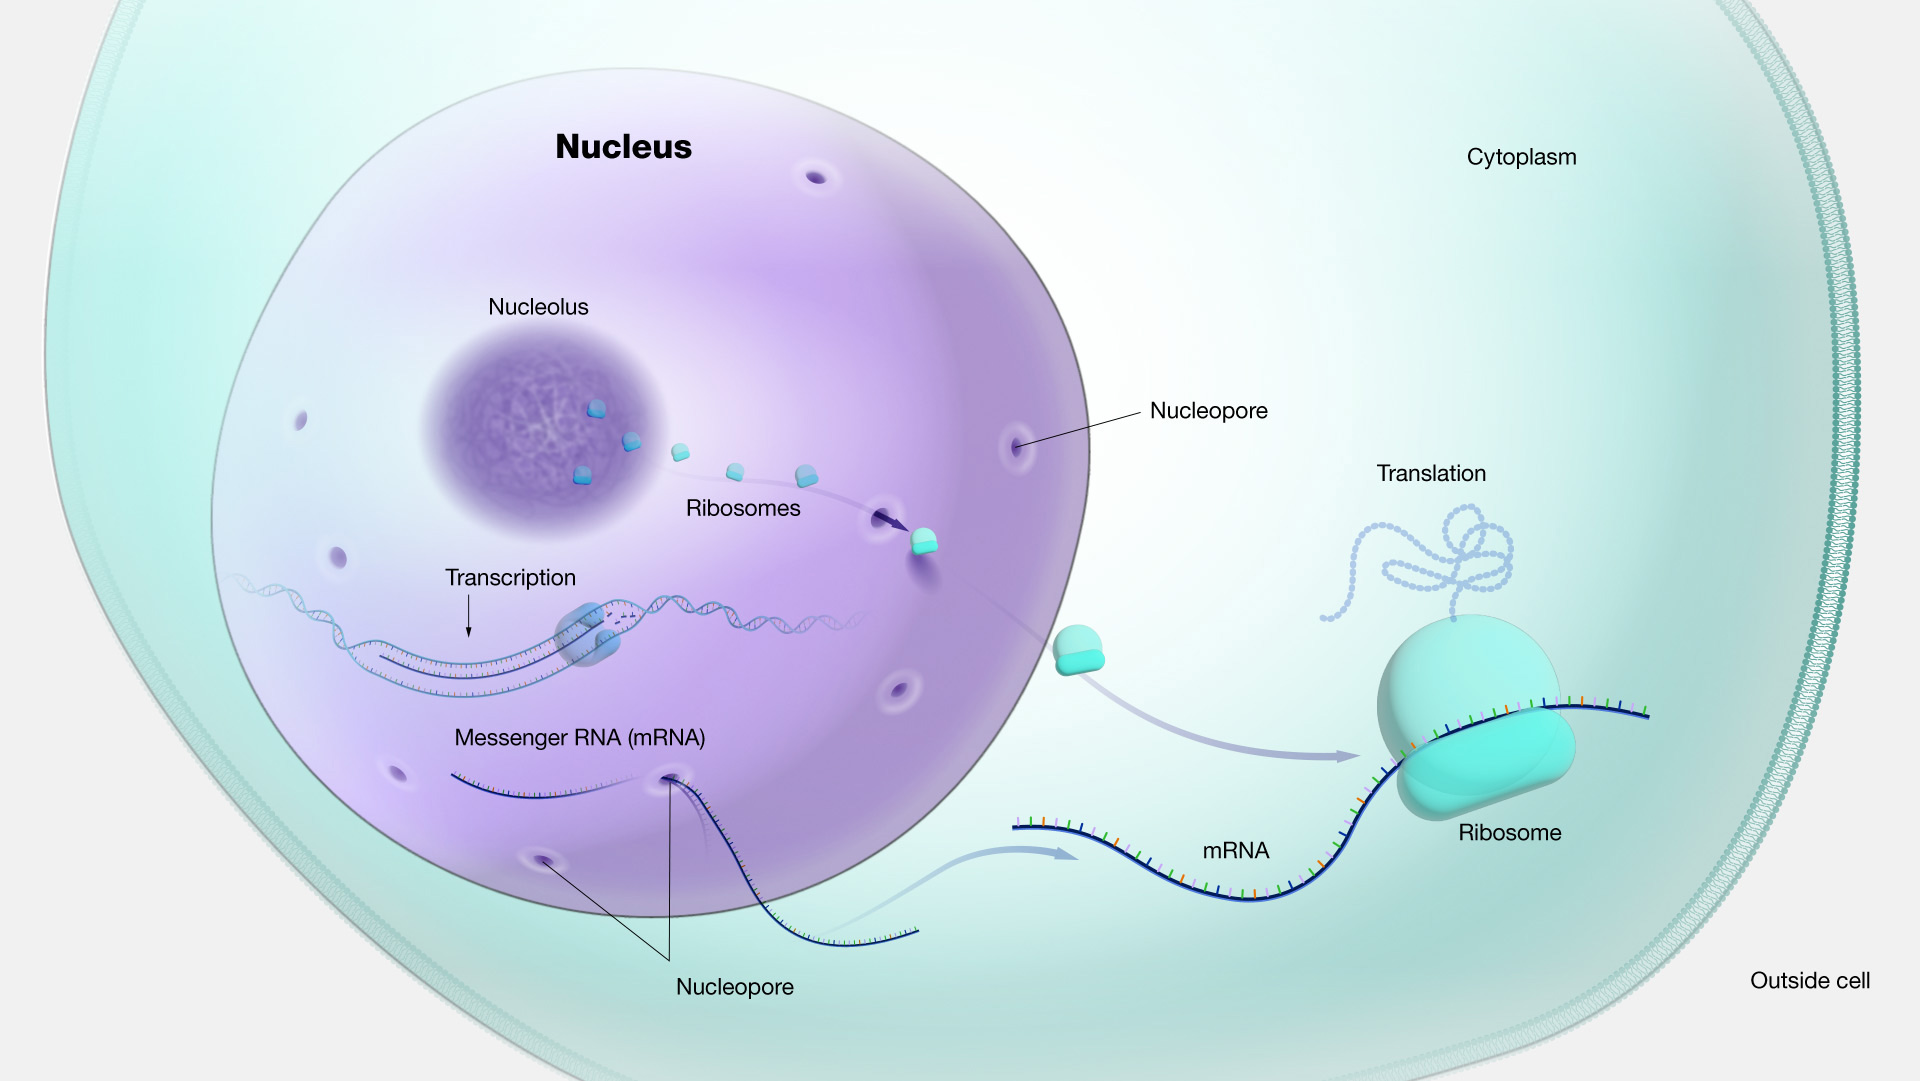
\includegraphics[width=\linewidth]{figures/nucleus.jpg}
\smallskip
{\scriptsize\color{Muted}典型有核细胞的简化示意，非显微照片。}
\end{column}
\end{columns}
\source{原讲义第 1--6 章。图片：\href{https://www.genome.gov/genetics-glossary/Nucleus}{NHGRI / Nucleus}，\href{https://www.genome.gov/about-nhgri/Policies-Guidance/Copyright}{Public domain}，等比缩放。}
\note{先用一页补齐最必要的基础。DNA 保存遗传信息，基因是其中具有功能的区段。细胞按照相关信息产生 RNA，这叫转录。部分 RNA，也就是 mRNA，进一步提供制造蛋白质的信息，这叫翻译，并不是 RNA 分子自己变成蛋白质。同一个人的多数有核体细胞，基因组大体相同，但使用哪些基因、使用到什么程度会不同。所以 RNA 的表达组合可以帮助我们判断细胞的身份和状态。不过，RNA 还受到降解和测量过程影响，不能直接等同于蛋白质的数量或功能。}
\end{frame}

% 04：50 秒
\begin{frame}{空间转录组保留表达与位置的关联}
\renewcommand{\arraystretch}{1.6}
\begin{tabularx}{\textwidth}{@{}lYY@{}}
\toprule
方法 & 主要信息 & 需要注意的限制\\
\midrule
Bulk RNA-seq & 混合组织的总体表达 & 难以区分各类细胞贡献\\
单细胞 RNA-seq & 细胞之间的表达差异 & 常规解离后通常丢失原位坐标\\
\textcolor{Teal}{空间转录组} & \textcolor{Teal}{RNA 表达及对应位置} & 测量单位可能是 cell、spot 或 bin\\
\bottomrule
\end{tabularx}
\key{分析前首先确认：一个观测位置代表什么？}
\small 一个 spot 可能覆盖多个细胞，网格边界也不自动等于细胞边界。
\source{原讲义第 7--9 章。}
\note{几种测量方式的区别，可以从保留了什么信息来理解。Bulk 把组织混在一起测，看到总体表达。单细胞测量尽量区分每个细胞，能够研究个体差异，但常规解离以后通常不知道它们原来在哪里。空间转录组把表达和位置关联起来，适合研究组织布局。不过空间分辨率和分析单位要具体看技术。有些数据对应细胞，有些对应 spot 或合并的 bin。一个 spot 可能含有多种细胞，这会直接影响后续任务和结果解释。}
\end{frame}

% 05：40 秒
\begin{frame}{把表达信号放回组织地图}
\centering
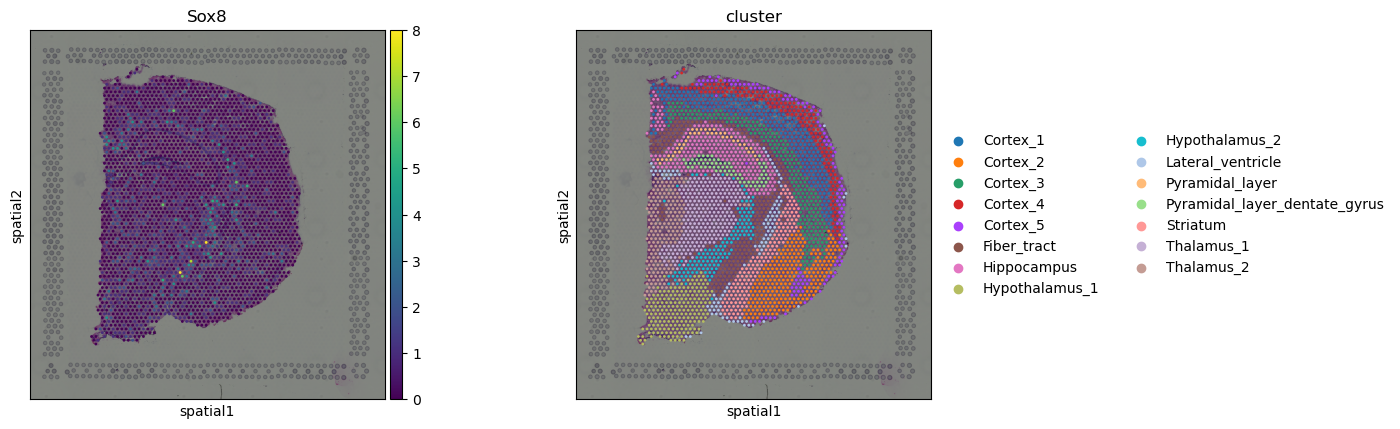
\includegraphics[width=.96\textwidth,height=4.45cm,keepaspectratio]{figures/spatial.png}
\par\smallskip
\raggedright
\small 左图：Sox8 表达信号。\quad 右图：分群及注释标签。
\par 同一组织位置可以承载表达值，也可以承载分析后的标签。
\source{原讲义第 8 章配图，来自\href{https://squidpy.readthedocs.io/en/latest/notebooks/examples/plotting/plot_scatter.html}{Squidpy 官方教程}，\href{https://github.com/scverse/squidpy/blob/main/LICENSE}{BSD 3-Clause}。此图不是肿瘤案例样本，点不自动等于单个细胞。}
\note{这张图直观展示了什么叫把表达放回组织地图。左边每个位置用连续颜色表示 Sox8 的表达信号，右边则把分群和注释标签画在相应位置。这样可以看到哪些表达特征集中在什么区域。需要区分两个层次：位置与分子信号来自实验，标签还经过分析和解释。这是讲义引用的官方教程图片，不是我们肿瘤案例的实验结果，也不能把图上每个点直接当作一个细胞。}
\end{frame}

% 06：65 秒
\begin{frame}{计算机中的数据：表达矩阵与空间坐标}
\begin{columns}[T,onlytextwidth]
\begin{column}{.47\textwidth}
\textbf{表达矩阵 $X$}\par\medskip
\renewcommand{\arraystretch}{1.3}
\begin{tabular}{@{}lrrr@{}}
\toprule
位置 & 基因 A & 基因 B & 基因 C\\\midrule
P1 & 30 & 2 & 5\\
P2 & 27 & 3 & 8\\
P3 & 3 & 28 & 4\\
P4 & 16 & 17 & 6\\\bottomrule
\end{tabular}
\end{column}
\begin{column}{.49\textwidth}
\textbf{坐标矩阵 $S$}\par\smallskip
$P1=(0,0),\ P2=(1,0)$\par
$P3=(0,1),\ P4=(1,1)$\par\medskip
\small
$X$：观测位置 $\times$ 基因。\par
$S$：观测位置 $\times$ 二维坐标。\par
用 spot ID 保证行对应，另可关联组织图像。
\end{column}
\end{columns}
\key{每个计数表示记录到的表达信号，不是基因数量}
\small P4 的混合信号不直接证明单个细胞具有两种身份。零值也不必然表示真实无表达。
\source{原讲义第 10--11 章。数值与坐标均为教学构造，不是真实实验数据。}
\note{从 CS 角度，核心就是特征矩阵加坐标。这里沿用讲义的四个位置、三个基因。每一行是一个观测单位，每一列是一个基因，数字是实验记录的表达计数。比如 P1 和 P2 的表达模式比较接近。P4 同时有 A 和 B 的信号，可能因为一个 spot 覆盖了多类细胞，不能据此断言一个细胞具有两种身份。右边坐标表记录真实位置，必须通过 spot ID 与表达矩阵对应。还要确认数据保存的是原始计数还是处理后的值。零首先表示没有记录到相应信号，不能直接判断生物学上完全没有表达。}
\end{frame}

% 07：60 秒
\begin{frame}{常见分析流程与每一步的作用}
\renewcommand{\arraystretch}{1.3}
\begin{tabularx}{\textwidth}{@{}lY@{}}
\toprule
步骤 & 主要目的\\\midrule
质量控制 & 检查低计数、异常观测及组织覆盖等问题\\
归一化与特征选择 & 缓解部分测量总量差异，选择有信息的基因\\
降维与聚类 & 提取主要表达模式，寻找相似群体\\
生物学注释 & 结合多个标志基因、参考数据与组织背景解释群体\\
空间分析 & 结合真实坐标研究区域、邻域与表达分布\\\bottomrule
\end{tabularx}
\key{聚类编号需要解释，UMAP 坐标需要与组织坐标区分}
\small 预处理应符合具体模型的输入要求。Scanpy 常用于表达分析，Squidpy 支持进一步的空间分析。
\source{原讲义第 12 章。}
\note{拿到数据以后，先检查质量，再按方法要求做预处理。归一化主要缓解部分测量总量差异，不能消除全部误差。特征选择和降维帮助提取主要模式，再用聚类发现相似群体。算法给出的 Cluster 0 或 Cluster 1 只是编号，具体是什么细胞或区域，需要结合标志基因和组织背景来注释。最后再使用真实坐标研究空间关系。这里特别要记住，UMAP 是表达特征的低维表示，图上的两个点靠近，不代表它们在组织里也靠近。不同模型对原始计数或归一化值的要求也可能不同。}
\end{frame}

% 08：55 秒
\begin{frame}{CS / AI 可以研究的代表性问题}
\renewcommand{\arraystretch}{1.55}
\begin{tabularx}{\textwidth}{@{}lYY@{}}
\toprule
生物问题 & 输入信息 & 算法输出\\\midrule
组织有哪些区域？ & 表达、坐标等 & 空间域标签\\
混合位置有什么细胞？ & 混合表达、参考数据 & 细胞类型组成或丰度估计\\
图像能否预测表达？ & 组织图像块 & 一组基因的预测表达\\
\bottomrule
\end{tabularx}
\medskip
\small 还可以研究空间变异基因，或结合配体受体知识提出候选通信关系。
\key{先明确生物问题与输出含义，再选择模型}
\source{原讲义第 13 章。预测表达属于推断，细胞组成指标需按具体方法定义解释。}
\note{讲义里介绍了几类计算任务。空间域识别回答组织有哪些表达或结构区域，可以对应聚类、表征学习等方法。反卷积处理混合 spot，估计其中不同细胞类型的组成，不过方法输出可能是丰度或 RNA 贡献，不能自动当成细胞数量比例。图像预测表达则可以看作多输出回归或多模态学习，但预测不能当作新完成的 RNA 实验。还有空间变异基因和候选细胞通信等问题。这些任务的输出各不相同，因此我理解最重要的是先把输入、输出和生物问题说清楚。}
\end{frame}

% 09：70 秒
\begin{frame}{案例：免疫细胞在肿瘤内部还是边缘？}
\begin{enumerate}\wideitems
\item \textbf{定义区域}：用有依据的图像标注等区分内部与边缘。
\item \textbf{推断组成}：根据测量单位选择注释或反卷积。
\item \textbf{明确比较指标}：比较密度、比例或方法定义的丰度。
\item \textbf{验证结果}：核对图像与标志信号，增加独立样本或实验。
\end{enumerate}
\medskip
\small 在能够按细胞计数的数据中：
\[
\text{免疫细胞密度}=\frac{\text{免疫细胞数}}{\text{区域面积}},\qquad
\text{免疫细胞比例}=\frac{\text{免疫细胞数}}{\text{区域总细胞数}}.
\]
\source{原讲义第 14 章。分母须大于零。RNA 贡献估计不能直接代入细胞数公式。此页为研究思路，无预设结论。}
\note{回到开头的问题，我们不能只把模型跑完、画一张图就结束。第一步要定义什么算肿瘤内部、什么算边缘，例如由专家根据组织图像标注。第二步根据测量单位选择方法，单细胞可以先注释，混合 spot 则需要考虑反卷积。第三步明确更多是什么意思：单位面积的免疫细胞密度更高，还是免疫细胞在全部细胞中的比例更高？这两个指标回答不同问题。如果模型只给出 RNA 相对贡献，就不能直接套用细胞计数公式。最后要回到图像与标志信号核对，并用独立样本或其他实验支持结论。}
\end{frame}

% 10：65 秒
\begin{frame}{科研结论需要匹配的验证证据}
\begin{itemize}\wideitems
\item \textbf{独立样本单位}：同一切片的数千个 spot 共享供体，不能等同于数千名患者。
\item \textbf{泛化范围}：想验证新患者效果，应按供体划分训练与测试数据。
\item \textbf{参照可靠性}：专家标注、独立实测与已有算法输出的证据强度不同。
\item \textbf{结论范围}：空间靠近或表达相关可以提出假设，机制解释还需要更多证据。
\end{itemize}
\source{原讲义第 15 章。数据划分应与研究目标一致，并检查预处理、参考构建和调参中的信息泄漏。}
\note{最后是从计算结果走向科学结论时容易忽略的地方。一张切片可以产生数千个位置，但它们来自同一个供体，不能当作几千个独立患者。如果想声称模型能用于新患者，就应该按供体划分训练和测试，而不是随机拆同一张切片上的相邻位置。验证时还要看参照是什么，已有算法的输出并不自动是真值。即使在切片上看到免疫细胞的位置差异，也只能先支持相应样本中的观察。进一步推广到患者群体，或者解释差异的原因，都需要相匹配的独立数据与实验设计。}
\end{frame}

% 11：25 秒。正文合计 600 秒。
\begin{frame}{目前的理解与下一步学习}
\begin{itemize}\wideitems
\item 空间转录组关联 \alert{RNA 表达与组织位置}。
\item 计算分析连接 \alert{表达矩阵、空间坐标与组织图像}。
\item 模型输出的生物学解释需要 \alert{明确的指标与验证证据}。
\end{itemize}
\vspace{5mm}
\textbf{下一步：}选取公开数据，练习基础分析，并检查表达矩阵与空间位置的对应关系。
\medskip
{\color{Muted}谢谢老师，欢迎指正。}
\note{这次整理以后，我的主要理解是：空间转录组把 RNA 表达和组织位置联系起来，计算分析则把矩阵、坐标和图像连接起来。真正进入科研，还要理解模型输出是什么，以及什么证据能够支持它。下一步我计划选一份公开数据练习基础分析，把这些概念与实际数据对应起来。谢谢老师。}
\end{frame}

% 附录不计入正文页数与十分钟讲述。
\appendix
\begin{frame}[noframenumbering]{附录：讲义中的延伸阅读}
\small
\begin{itemize}\wideitems
\item \href{https://www.genome.gov/genetics-glossary}{NHGRI 基础术语}：DNA、RNA、转录、翻译与基因表达。
\item St\aa hl 等，2016，\textit{Science}：\href{https://www.science.org/doi/10.1126/science.aaf2403}{空间转录组原始研究}。
\item \href{https://anndata.readthedocs.io/en/stable/generated/anndata.AnnData.html}{AnnData} 与 \href{https://scanpy.readthedocs.io/en/stable/tutorials/basics/clustering.html}{Scanpy}：数据对象与基础分析。
\item Palla 等，2022，\textit{Nature Methods}：\href{https://www.nature.com/articles/s41592-021-01358-2}{Squidpy 空间分析框架}。
\item Kleshchevnikov 等，2022，\textit{Nature Biotechnology}：\href{https://www.nature.com/articles/s41587-021-01139-4}{cell2location 细胞组成推断}。
\end{itemize}
\source{内容依据用户修改后的入门讲义。此页供提问和后续阅读，正常汇报可在上一页结束。}
\end{frame}
\end{document}
